% !TEX root = ../main.tex

% Indicate the main file. Must go at the beginning of the file.

%-------------------------------------------------------------------------------
% CHAPTER TEMPLATE
%-------------------------------------------------------------------------------


\chapter{Theoretische Grundlagen} % Main chapter title
\label{Chapter2TheoretischeGrundlagen} % Change X to a consecutive number; for referencing this chapter elsewhere, use \ref{ChapterX}
Der MVB ist ein in der Bahnindustrie verbreiteter Fahrzeugbus, welcher auf dem Prinzip \textit{single master - multiple slaves} aufbaut. In folgenden Abschnitten werden die Grundlagen des Busses aufgezeigt. Alle Daten und Abbildungen in folgendem Kapitel wurden, wenn nicht anders deklariert, aus der Norm IEC 61375-3-1 entnommen. \cite{MVB_Norm} 

%--------------------------------------------------------------------------------
% SECTION "Multifunction Vehicle Bus"
%--------------------------------------------------------------------------------

\section{Multifunction Vehicle Bus}

%\textcolor{red}{Einführung in Grundbegriffe und das Konzept MVB, In der Regel ist zumindest ein kurzes Theoriekapitel notwendig. Es nimmt Bezug  auf das thematische Oberthema, aber natürlich nicht auf allgemeine theoretische Grundlagen etwa aus der Naturwissenschaft.}
%\textcolor{red}{Vlt noch ergänzen optisch und elektrische(EMD, ESD)Ausführungen und bei Sicherheitskritischen Anwendungen (nicht Komfort) meist Redundant geführt Linie A und B..}

Der Abschnitt beleuchtet die wesentlichen Aspekte des Physical und Link Layers des Datenbusses gemäss der Norm SN EN 61375. Der Fokus liegt auf der Datenübertragungsgeschwindigkeit, dem Bit-Encoding und den Steuermechanismen wie den Start-Delimitern und dem Master-Slave-Prinzip. Neben den technischen Grundlagen, wie der Manchester-Kodierung und den Non-Data-Symbolen, wird die Struktur von Frames und Telegrammen detailliert beschrieben.

Nachfolgende Texte sowie Illustrationen sind alle aus der Norm SN EN 61375-3-1 Kapitel 


%-----------------------------------
% SUBSECTION "MVB Bus"
%-----------------------------------

%\textcolor{red}{MVB Aufbau, Master Slave Prinzip, Telegrammme, F-Codes}
\subsection{Linklayer - Master-Frame}
\label{sub:MasterFrame}
Das Master-Frame ist der Anfang eines Telegrammes und wird immer vom Busmaster gesendet. Nach dem Startbit folgen 8 Bit, welche dem Master-Frame Delimiter in Abbildung \ref{fig:FrameDelimiterMasterSlave} entsprechen. 

\begin{figure}[H]
    \centering
    \begin{minipage}{0.33 \textwidth}
        \centering
        \begin{enumerate}
            \item Master Start-Delimiter
            \item 16 Bit Frame Data
            \begin{enumerate}
                \item F-Code: 4 Bit
                \item Data: 12 Bit
            \end{enumerate}
            \item 8 Bit check sequenze 
            \item End-Delimiter
        \end{enumerate}
    \end{minipage}
    \hfill
    \begin{minipage}{0.65 \textwidth}
        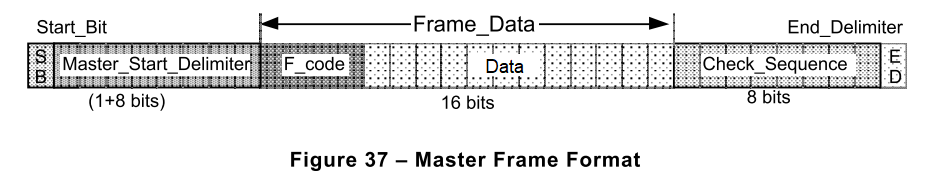
\includegraphics[width = \textwidth]{Figures/Chap2/Grundlagen/MVB_DOKU/Frames und Telegramme/Fig37_MasterFrameFormat.png}
        \caption{Master-Frame Format}
        \label{fig:MasterFrameFormat}
    \end{minipage}
        
\end{figure}

\subsection{Linkayer - Slave-Frame}
\label{sub:SlaveFrame}
Das Slave-Frame folgt direkt nach dem Master-Frame, sofern der angesprochene Slave eingeschalten und sendefähig ist. Ansonsten würde der Master nach einer definierten maximalen Wartezeit ein neues Telegramm beginnen. \newline
Im Gegensatz zum Master-Frame hat der Slave-Frame verschiedene Längen, je nach F-Code. Je nach Grösse werden ebenfalls mehrere Check-Sequenzen geschickt. Eine Check-Sequenz kann dabei bis zu 64 Bit verifizieren.

\begin{enumerate}
    \item Slave Start-Delimiter (8 Bit)
    \item 16 - 256 Bit Frame Data (individuell)
    \item Check sequence nach maximal 64 Bit Daten 
    \item End-Delimiter
\end{enumerate}

\begin{figure}[H]
    \centering
    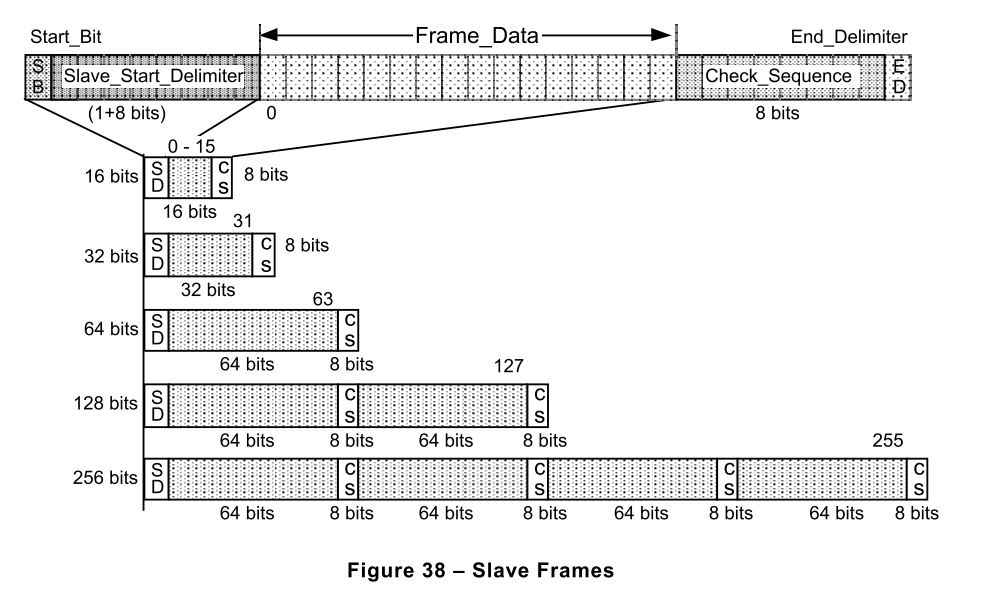
\includegraphics[width = 0.8 \textwidth]{Figures/Chap2/Grundlagen/MVB_DOKU/Frames und Telegramme/Fig38_SlaveFrameFormat.png}
    \caption{Slave-Frame Format}
    \label{fig:SlaveFrameFormat}
\end{figure}

\subsection{Linklayer - Check Sequence}
\label{sub:CheckSequenz}
Die Prüfsequenz wird als zyklische Redundanzprüfung (CRC) für die 16, 32 oder 64 Bit an Daten berechnet, welche gemäss dem generativen Polynom in Gleichung \ref{equ:GenerativesPolynom} berechnet werden soll.

\begin{equation}
    G(x) = x^7 + x^6 + x^5 + x^2 + 1
    \label{equ:GenerativesPolynom}
\end{equation}

\subsection{Link Layer - Master / Slave Prinzip}
\label{sub:MasterSlavePrinzip}
Der MVB wird mit ein Master - Slave Prinzip realisiert. Der Master fordert mit einem definierten \textit{Master\_Frame} (Kapitel \ref{sub:MasterFrame}) die Daten der jeweiligen Slave-Teilnehmer an. Der Slave beantwortet die Anfrage mit einem \textit{Slave\_Frame} (Kapitel \ref{sub:SlaveFrame}. Das Master- und Slave-Frame bilden zusammen ein Telegram (Siehe Abbildung \ref{fig:Fig39_Telegamm_definition.png}). 

\begin{figure}[H]
    \centering
    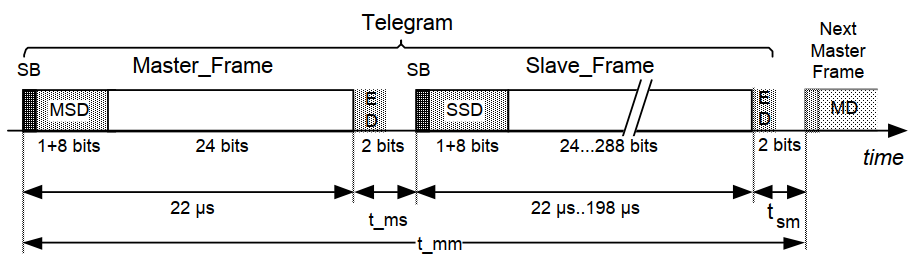
\includegraphics[width=0.85\linewidth]{Figures/Chap2/Grundlagen/MVB_DOKU/Frames und Telegramme/Fig39_Telegamm_definition.png}
    \caption{Master- und Slave-Frame bilden ein Telegram}
    \label{fig:Fig39_Telegamm_definition.png}
\end{figure}

In der Norm \textit{SN EN 61375} sind die Telegramme in 16 verschiedene Frame-Codes (F-Codes) unterteilt. In Abbildung \ref{fig:FCodeListe} ist eine tabellarische Auflistung zu sehen. 

\begin{figure}[H]
    \centering
    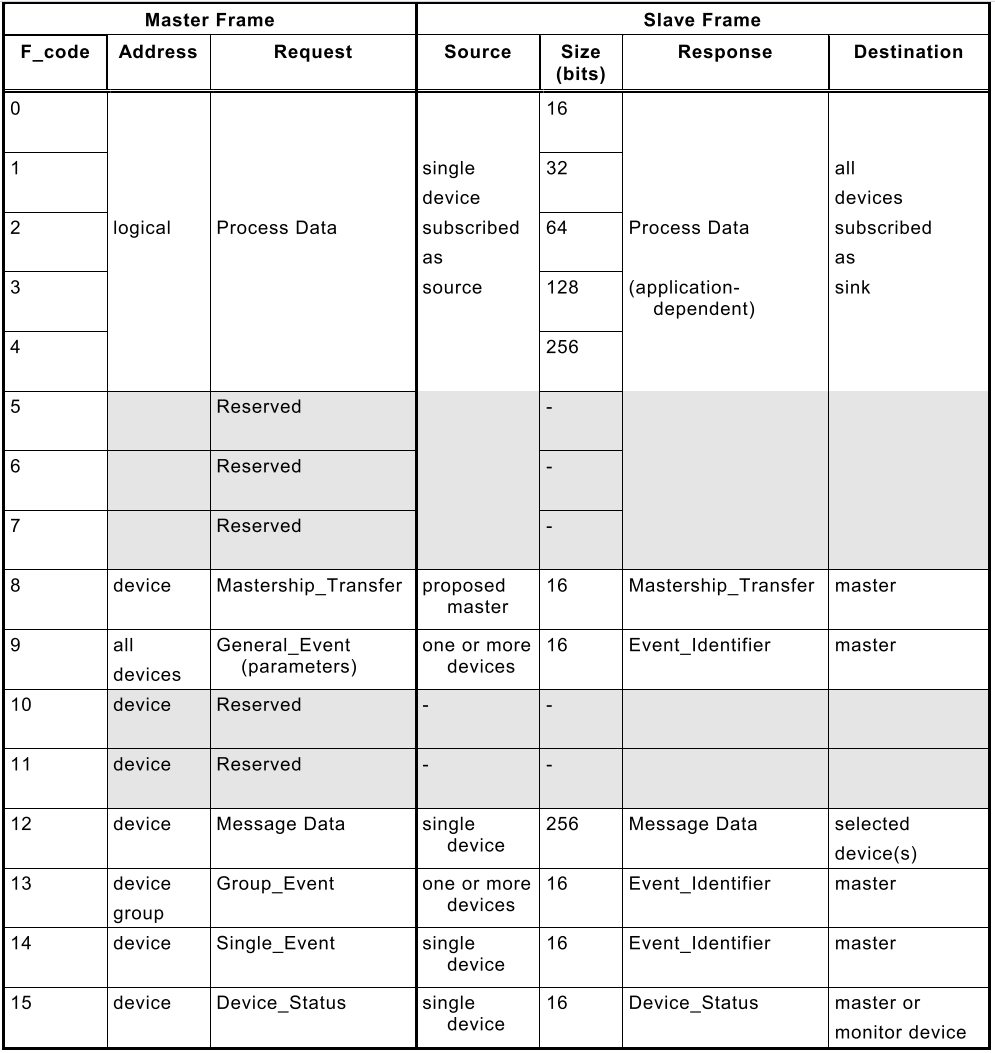
\includegraphics[width=0.9\linewidth]{Figures/Chap2/Grundlagen/MVB_DOKU/Frames und Telegramme/F-Code Liste.png}
    \caption{Auflistung aller möglichen F-Codes}
    \label{fig:FCodeListe}
\end{figure}

\subsection{Physical Layer - Geschwindigkeit auf dem Datenbus}
\label{sub:GeschwindigkeitDatenbus}
Die Signalgeschwindigkeit ist in der Norm \textit{SN EN 61375-3-1:2012 Kap. 4.3.1} definiert. Diese lautet 1.5 MBit/s $\pm$ 0.01\% mit Manchester Encoding (siehe \ref{sub:BitEncoding})

\begin{itemize}
  \item BR (Bitrate): 1.5 MHz oder 1.5 MBit/s
  \item BT (Bittime): 666.7 ns
\end{itemize}

\subsection{Physical Layer - Bit-Encoding}
\label{sub:BitEncoding}
Die Frame-Data sollen gemäss folgender \textit{Bit-Encoding} (Abb. \ref{fig:manchester_Bit_Encoding}) kodiert werden.

\begin{itemize}
    \item Eine "'1"' soll kodiert werden als ein \textbf{HIGH} in der ersten und dann ein \textbf{LOW} in der zweiten Hälfte des Bit
    \item Eine "'0"' soll kodiert werden als ein \textbf{LOW} in der ersten und dann ein \textbf{HIGH} in der zweiten Hälfte des Bit
\end{itemize}

\begin{figure}[H]
    \centering
    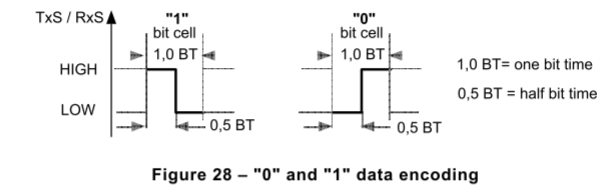
\includegraphics[width = 0.7 \textwidth]{Figures/Chap2/Grundlagen/MVB_DOKU/Layer/Bit_Encoding.png}
    \caption{Machester Bit-Encoding}
    \label{fig:manchester_Bit_Encoding}
\end{figure}

\subsection{Physical Layer - Non Data Symbols} 
\label{sub:NonDataSymbols}
Der Start-Delimiter enthält \textit{Non Data Symbols}, welche zur Synchronisierung verwendet werden. Diese Symbols werden ebenfalls \textit{Manchastercode violations} genannt. Folgende Liste zeigt, wie die Symbols (Abb. \ref{fig:NonDataSymbolsEncoding}) kodiert sind

\begin{itemize}
    \item "'NH"' soll kodiert werden als ein \textbf{HIGH} Signal während eines Bit 
    \item "'NL"' soll kodiert werden als ein \textbf{LOW} Signal während eines Bit
\end{itemize}

\begin{figure}[H]
    \centering
    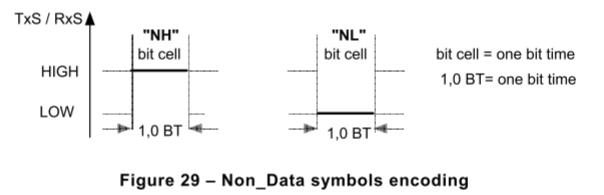
\includegraphics[width = 0.7 \textwidth]{Figures/Chap2/Grundlagen/MVB_DOKU/Layer/Non_Data_Symbol.png}
    \caption{Non Data Symbols encoding}
    \label{fig:NonDataSymbolsEncoding}
\end{figure}

\subsection{Physical Layer - Start-Delimiter}
\label{sub:StartDelimiter}
Der Start-Delimiter hat die Funktion ein Frame eindeutig zu identifizieren. Hierbei gibt es zwei unterscheidbare Start-Delimiter, der \textit{Master-Frame Delimiter} und der \textit{Slave-Frame Delimiter}. In Abbildung \ref{fig:FrameDelimiterMasterSlave} sind beide Start-Delimiter aufgezeigt. Diese Abbildung stammt aus der MVB Case Study der EPFS und ist in Anhang \ref{app:File11} auf Seite 29 zu finden. Gut zu sehen sind die in Kapitel \ref{sub:NonDataSymbols} erwähnten Manchester Violations beim Master-Frame Delimiter an Stelle 1, 2, 4 und 5 und beim Slave-Frame Delimiter an den Stellen 4, 5, 7 und 8. Das gelb markierte \textit{Start Bit} ander der Stelle 0 hat die Funktion den Start nach einer unbestimmten Zeit im Zustand \textit{Idle} zu signalisieren. Dies gehört nicht zum Start-Delimiter (siehe Abbildung \ref{fig:MasterFrameFormat} und \ref{fig:SlaveFrameFormat}). Die Manchester decodierten Start-Delimiter sind somit wie folgt aufgebaut:

\begin{itemize}
    \item Master-Frame Delimiter: [NH, NL, 0, NH, NL, 0, 0, 0]
    \item Slave-Frame Delimiter: [1, 1, 1, NL, NH, 1, NL, NH]
\end{itemize}


\begin{figure}[H]
    \centering
    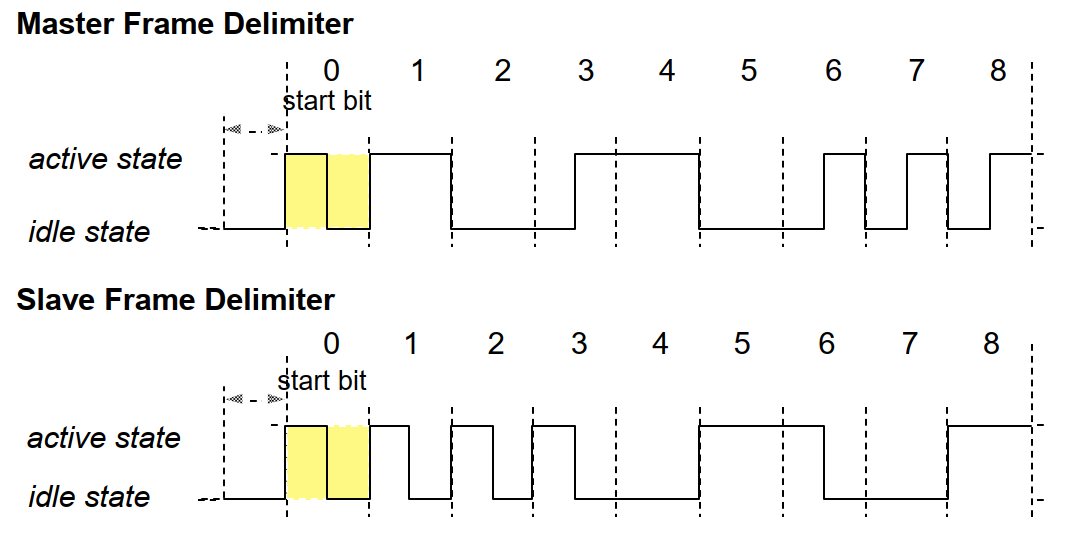
\includegraphics[width=0.8\linewidth]{Figures/Chap2/Grundlagen/MVB_DOKU/Layer/Frame_Delimiter.png}
    \caption{Illustration Master- und Slave-Frame Delimiter}
    \label{fig:FrameDelimiterMasterSlave}
\end{figure}

\section{Übertragungsmedien}
\label{Übertragungsmedien}

Für den MVB sind in der Norm \textit{SN EN 61375-3-1 Kapitel 4.4 bis 4.6 } drei Varianten definiert. Diese sind wie folgt:
\begin{itemize}
    \item \textbf{ESD:} Electrical Short Distance Bus
    Über eine Signalleitung mit Potenzialtrennung mit Optokoppler oder ohne Potenzialtrennung
    \item  \textbf{EMD:} Electrical Middle Distance Bus
    Über verdrillte Signalleitung und Potenzialtrennung über Induktivität
    \item  \textbf{OGF:} Optical Glass Fiber
    Über ein Lichtwellenleiter
\end{itemize}

In Abbildung \ref{fig:TransceiverInterface} ist eine Illustration der drei Übertragungsmedien gezeigt. 

\begin{figure}[H]
    \centering
    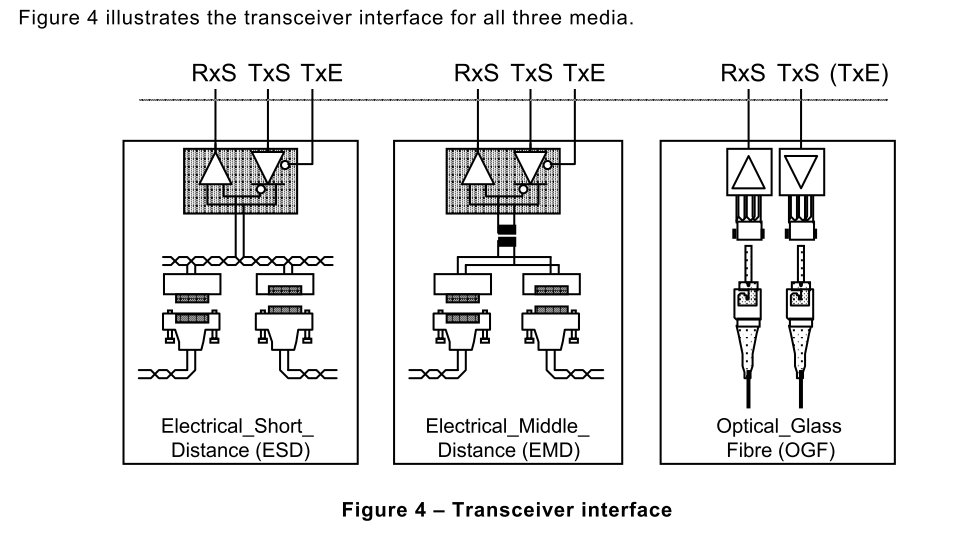
\includegraphics[width=0.9\linewidth]{Figures/Chap2/Grundlagen/MVB_DOKU/EMD_ESD_OGF/Fig4_Transceiver interface.png}
    \caption{Transceiver Interfaces}
    \label{fig:TransceiverInterface}
\end{figure}

Die Verbindungen zwischen ESD und EMD erfolgen über einen D-Sub9-Stecker. Tabelle \ref{tab:PinESDEMD} zeigt die Pinbelegung der Stecker sowie deren Funktionen. Dabei wird zwischen \textit{A Bus} und \textit{B Bus} unterschieden, da der MVB redundant geführt ist und auf den jeweiligen Leitungen A und B gespiegelt wird. Die Details zur Redundanz werden nicht weiter behandelt.


\begin{table}[H]
    \centering
    \begin{tabular}{|r||c|c|} \hline
        Pin & ESD & EMD\\ \hline
        1 & A Data Positiv & A Data Positiv\\ \hline
        2 & A Data Negativ & A Data Negativ\\ \hline
        3 & TxE (optional) & TxE (optional)\\ \hline
        4 & B Data Positiv & B Data Positiv\\ \hline
        5 & B Data Negativ & B Data Negativ\\ \hline
        6 & A Bus Ground & A Positiv Pole\\ \hline
        7 & B Bus Ground & A Negativ Pole\\ \hline
        8 & A Bus 5V & B Positiv Pole\\ \hline
        9 & B Bus 5V & B Negativ Pole\\ \hline
    \end{tabular}
    \caption{Pinbelegung für ESD und EMD Stecker}
    \label{tab:PinESDEMD}
\end{table}

Für das Übertragungsmedium OGF ist keine Pinbelegung erforderlich, da zwei separate Lichtwellenleiter verwendet werden: Einer dient zum Senden, der andere zum Empfangen von Signalen.